\documentclass[a0paper,portrait]{xebaposter}

\usepackage[utf8]{inputenc}
\usepackage[T1]{fontenc}
\usepackage{fontspec}
\usepackage[english]{babel}

\usepackage{caption}
\captionsetup{
  font=small,
  labelfont=bf
}

\usepackage{array,booktabs}
\usepackage{amsmath}
\usepackage{amssymb}

\usepackage{graphicx}
\graphicspath{{figures/}}

\usepackage[style=apa,backend=biber]{biblatex}
\addbibresource{reference.bib}

\usepackage{lipsum}

\selectcolormodel{RGB}
\definecolor{zjublue}{RGB}{0,62,135}
\definecolor{zjugrey}{RGB}{230,230,230}

\addto{\captionsenglish}{
  \renewcommand{\refname}{\vspace{-0.7em}}
  \renewcommand{\figurename}{Fig.}
}

\begin{document}

\begin{poster}
  {
    grid=false,
    columns=2,
    eyecatcher=true,
    borderColor=zjublue,
    headerheight=0.1\textheight,
    headerborder=closed,
    headershape=smallrounded,
    headerColorOne=zjublue,
    headerColorTwo=white,
    headershade=plain,
    headerFontColor=white,
    headerfont=\large\bf\setmainfont{Impact},
    textborder=roundedsmall,
    boxColorOne=white,
    linewidth=1pt,
    boxpadding=1em
  }
  {
    
\includegraphics[height=0.75\headerheight]{zju-logo.png}
  }
  {
    \color{zjublue}\bf\huge
    Poster Theme for Department of Psychology and Behavioral Sciences Undergraduate Students' Poster Exibition
  }
  {
    \color{zjublue}
    Made by Shuoan Li

    Department of Psychology and Behavioral Science, Zhejiang University
  }

  \begin{posterbox}[name=introduction,span=2,column=0,row=0]{Introduction}
    \begin{minipage}{.48\textwidth}
      \lipsum[1]

      \vspace{.01\textheight}
      \setlength\fboxsep{.05\textwidth}
      \colorbox{zjugrey}{\parbox{.9\textwidth}{
        \section*{Present question}
        \lipsum[2]
        \vspace{.01\textheight}
      }}
    \end{minipage}\hspace{.02\textwidth}
    \begin{minipage}{.48\textwidth}
      \lipsum[3-4]
    \end{minipage}
  \end{posterbox}

  \begin{posterbox}[name=exp1,column=0,below=introduction]{Experiment 1}
    \lipsum[5]
  \end{posterbox}

  \begin{posterbox}[name=exp2,column=1,below=introduction]{Experiment 2}
    Here is a table.
    
    \vspace{.01\textheight}
    \begin{center}
    \begin{tabular}{c c c}
      \toprule
      header 1 & header 2 & header 3\\
      \midrule
      data (1,1) & data (1,2) & data (1,3)\\
      data (2,1) & data (2,2) & data (2,3)\\
      data (3,1) & data (3,2) & data (3,3)\\
      \bottomrule
    \end{tabular}
    \captionof{table}{Example table}
    \end{center}
  \end{posterbox}

  \begin{posterbox}[name=exp3,column=0,below=exp1,above=bottom]{Experiment 3}
    Here is an image.
    
    \begin{center}
      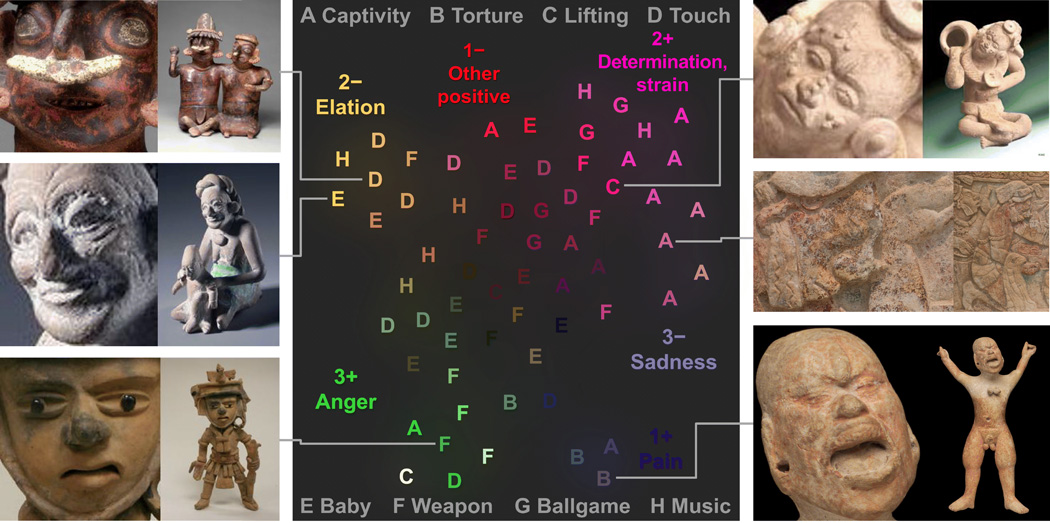
\includegraphics[width=\textwidth]{abb1005-f4.jpeg}
      \captionof{figure}{This is a figure\parencite{Cowen2020UniversalFE}}
    \end{center}
  \end{posterbox}

  \begin{posterbox}[name=discussion,column=1,below=exp2]{Discussion}
    \lipsum[8]
  \end{posterbox}

  \begin{posterbox}[name=reference,column=1,below=discussion]{Reference}
    \printbibliography[heading=none]
  \end{posterbox}

  \begin{posterbox}[name=contact,column=1,below=reference,above=bottom]{Contact}
    Further question or comments, please contact

    Shuoan Li at 3220101015@zju.edu.cn
  \end{posterbox}

\end{poster}

\end{document}
